
\documentclass[11pt]{article}

\usepackage[utf8]{inputenc}
\usepackage[ngerman]{babel}
\usepackage{csquotes}

\usepackage{fullpage}
\usepackage{setspace}
\usepackage{parskip}
\usepackage{titlesec}
\usepackage{mathptmx}
\usepackage{comment}

\usepackage{graphicx}
\usepackage[section]{placeins}
\usepackage[justification=centering]{caption}
\usepackage{wrapfig}

\usepackage{authblk}
\usepackage{hyperref}


\PassOptionsToPackage{
style=apa,
doi=false,
isbn=false,
eprint=false
}{biblatex}
\usepackage[backend=biber]{biblatex}
\addbibresource{ws1819_skribbl.bib}

\PassOptionsToPackage{hyphens}{url}

\makeatletter

\renewenvironment{abstract}
{{\bfseries\noindent{\abstractname}\par\nobreak}\footnotesize}
{\bigskip}

\renewenvironment{quote}
  {\begin{tabular}{|p{13cm}}}
  {\end{tabular}}

\titlespacing{\section}{0pt}{*3}{*1}
\titlespacing{\subsection}{0pt}{*2}{*0.5}
\titlespacing{\subsubsection}{0pt}{*1.5}{0pt}

\begin{document}

\begin{titlepage}
   \begin{center}
       \vspace*{1cm}

       \Huge
       Skribbl.AI Projektdokumentation (IQ vs. KI)
       \vspace{1.5cm}

       
\includegraphics[width=0.4\textwidth]{images/logo_htw.jpg}

       \vspace{1.0cm}
       
\includegraphics[width=0.2\textwidth]{images/logo_skribbl.png}
       \vspace{1.0cm}

       \LARGE

       Josefine Sophie Busch, Malin Dulkies, Rachel Escueta, Tim-Niklas Heise, Ninoslav Kjireski, Anastasia Litvina, Anh Quang Vu-Tuyen

       \vfill

       Projektarbeit \\

       \vspace{0.8cm}

       Hochschule für Technik und Wirtschaft\\
       Berlin\\

   \end{center}
\end{titlepage}

       Prof. Dr. Klaus Jung\\
       Wintersemester 2018/2019\\
\pagebreak
\tableofcontents
\pagebreak
\listoftables
\listoffigures
\pagebreak

\section{Einleitung}
\label{chap: Einleitung}
\subsection{Leitfaden}
\label{chap: leitfaden}
\begin{wrapfigure}{R}{0.3\textwidth}
\centering

\includegraphics[width=0.25\textwidth]{images/logo_skribbl.png}
\caption{\label{fig:skribblLogo}Skribbl.AI Logo}
\end{wrapfigure}
Die Idee begann mit IQ gegen KI. Mit dem Einfall, was würde eigentlich passieren, wenn eine künstliche Intelligenz ein von einem Menschen gemaltes Bild  erkennen sollte? \\
Neuronale Netzwerke erbringen beeindruckende Leistungen bei der Erkennung fotorealistischer Aufnahmen. Sie helfen sogar Pathologen bei der Erkennung von Krebszellen \parencite{ElizabethDougherty2018}.\\
Was also würde  passieren, wenn wir eine künstliche Intelligenz mit den Kritzeleien einer Student*in konfrontieren?
 
\subsection{Aufbau des Projektes}
\label{chap: Aufbau}

Das Semesterprojekt ist ein Pflichtmodul des Studiengang Internationale Medieninformatik der HTW Berlin, welches im 5. Semester angesetzt ist. \\
In einer Gruppe von fünf bis acht zufällig gewählten Studierenden werden Konzepte entwickelt und dann in Anwendungen umgesetzt. Dabei stehen Themen aus Bereichen der Wirtschaft oder aus einem der verschiedenen Forschungsbereiche des Studienganges zur Wahl, an denen die Studierenden arbeiten können.

Die Studierenden werden dabei von einer Lehrkraft bzw. einer verantwortlichen Person aus dem wirtschaftlichen Unternehmen betreut.
Das Projekt ist in drei Bereiche unterteilt.

\subsubsection{ Themenvergabe und Konzeptausarbeitung }
\label{chap: Themenvergabe}

Unser Projekt ist das Projekt KI vs IQ, welches von Prof. Jung betreut wurde.
Die Vorgabe war, eine spielerische Anwendung zu entwickeln, in der ein Mensch gegen ein neuronales Netz antritt, welches dazu trainiert wurde, Bilder zu erkennen.

Mehr dazu in \autoref{chap: Grundlagen}
	
\subsubsection{  Projektmanagement }
\label{chap: Projektmanagement}
Die Belegung des Semesterprojektes erfolgt mit einer automatischen Belegung des Projektmanagement Moduls, welches agile Methoden im Allgemeinen und Scrum im Speziellen vermittelt. Dem entsprechend und der Tatsache zugrundeliegend, dass einige Gruppenmitglieder bereits Erfahrung mit Scrum hatten, haben wir uns dafür entschieden, im Projekt mit Scrum zu arbeiten beziehungsweise mit einer unseren Bedürfnissen und Gegebenheiten angepassten Version von Scrum.\\
Als unterstützende Werkzeuge für das Projektmanagement haben wir Trello und zum Gruppenmanagement beziehungsweise für die Kommunikation in der Gruppe Slack genutzt.

\subsubsection{ Durchführung }
\label{chap: durchfuhrung}
Die Durchführungsphase setzt sich dann konkret mit der Entwicklung der Anwendung auseinander. Wir entschieden uns dafür eine Website für unser Spiel zu bauen. Wir haben HTML 5, CSS 3, Sass 1.16.1 und Javascript Ecmascript 3 für das entwickeln der Webumgebung und des Spieles genutzt. Das neuronale Netzwerk ist ein TensorFlow 1.12.0 Model mit Keras 2.2.2, welches wir mit TensorFlow.js in unsere Webseite einbinden und mit Python 3 trainieren.\\
Mehr dazu in \autoref{chap: Anforderungen}

\section{Grundlagen}
\label{chap: Grundlagen}
\subsection{Design}
\subsubsection{Findung und Sketcher}

Wissend, dass wir ein Spiel kreieren wollten, welches sowohl Bilderkennung durch ein neuronales Netzwerk garantiert als auch den Spielspaß für den Spieler, galten unsere ersten Überlegungen dem Namen sowie Konzept des Spiels.
Abgeleitet von dem englischen Verb 'to scribble' mit ein paar Änderungen um den Namen für das deutsche Publikum besser aussprechbar zu machen, wurde 'Skribbl'. Das Kürzel '.AI' hingegen war für uns als Team sehr offensichtlich. Nicht nur wäre es eine wundervolle URL, sollte das Projekt zu einem späteren Zeitpunkt veröffentlicht werden, sondern sie zeigt ebenfalls die nahe Verbindung zu unserem neuronalen Netzwerk.

Folgend kam die Entscheidung dahingehend, was für eine Art von Spiel wir erschaffen wollten. Eine Zeichnung sollte erkannt werden. Natürlich gab es zahlreiche Konzeptideen, so mussten wir uns auf ein Konzept einigen. Dabei hatten wir von Anfang an direkt 3 verschiedene Implementierungen, die uns einfielen. Alle angelehnt an das selbe Konzept und dennoch von Grund auf verschieden, was den Spielspaß anging. Sollten die Spieler sehen, welche Ergebnisse das neuronale Netz aus der Zeichnung vorhersagte, oder sollten sie komplett im Dunklen stehen? Sollte es eine Überraschung werden oder nicht? Vielleicht etwas in der Mitte?

Während der Anfangsphase des Projektes und bei der Rechercher stießen wir auf ähnliche Konzepte, die ebenfalls eine Bilderkennung mit Zeichnungen implementierten. Besonders hervorzuheben wären hier Sketcher \parencite{sketcher}, welches eine große Hilfe und Inspiration für uns war. Besonders hilfreich war auch das Tutorial von Zaid Alyafeai zu Sketcher \parencite{sketcherTutorial}. Außerdem gibt es auch ein Projekt von Google \parencite{quickDraw}.

\subsubsection{Mobile First}

Ein solches Projekt, mit Spiel-Charakter, wie man sie aus jedem App-Store kennt; kurze Level für ein Kurzweiliges Spielerlebnis machten eines schnell klar: Unsere Priorität lag auf Mobile-First.
Dabei mussten mögliche Hürden mit dem Touchscreen, den unterschiedlichen Bildschirmgrößen sowie Funktionen der verschiedenen Browser und Betriebssysteme erwartet werden. Dennoch war es für uns keine schwere Entscheidung den Desktop vorerst außen vor zu lassen und sicher zu stellen, dass unser Spiel optimal auf einem Smartphone spielbar ist.

\subsubsection{Accessibility}

Accessibility war ein Punkt, der zwar erst ein wenig später in unserem Projekt angesprochen wurde, aber dennoch von hoher Bedeutung für uns war. Mit dem sehr visuellen Thema des Zeichnens und der heutigen Einstellung zu Accessibility Themen, war uns schnell klar, dass wir unser Spiel so zugänglich wie möglich für alle Nutzer machen wollten.

Ein Styleguide wurde erstellt, in welchem jede Farbe und Schriftgröße so getestet wurde, dass sie den Werten des AA Standards der W3C Verordnung entspricht. Außerdem nahmen wir noch andere Richtlinen wie Clean Coding Regeln in unseren Styleguide mit auf.\\
Mehr dazu in \autoref{chap: Anlagen} 

\subsection{Frontend}
\subsection{Neuronales Netzwerk}
\subsubsection{Dataset}
Das Datenset mit dem wir unser neuronales Netzwerk trainiert haben ist das "Quick, Draw!" \parencite{quickDraw} Datenset, welches von Google zur Verfügung gestellt wird. Die Daten wurden durch Googles "Quick, Draw!" \parencite{quickDraw} gesammelt, in welchem Spieler Strichzeichnung von verschiedensten Dingen anfertigen müssen. Das Datenset in seiner Gänze besteht aus 345 Kategorien, mit mehr als 59 Millionen Zeichnungen. 
Wir haben uns dafür entschieden, die Daten im .npy Format zu nutzen, welche bereits auch so im Google-Bucket zur Verfügung standen. Das .npy Format stellt die Bilder in 28x28 Pixeln zur Verfügung. 
Für unser Modell haben wir uns für 100 ausgewählte Kategorien entschieden, mit jeweils 20.000 Bildern.
\section{Anforderungen}
\label{chap: Anforderungen}
\subsection{Produkt Vision}
\label{chap: productVision}
Unsere Produkt Vision ist, bis zum Ende des Wintersemesters 2018/2019 ein kurzweiliges Mini-Malspiel mit einem Einzelspielermodus entwickelt zu haben. Es soll speziell für mobile Endnutzer aller Altersklassen konzipiert sein.
\subsubsection{Die Kurzweiligkeit}
Die Kurzweiligkeit unseres Spiels ist offensichtlich eine der Eigenschaften, die am schwierigsten einzuschätzen sind. Um dennoch dieses Ziel nicht aus den Augen zu verlieren, einigten wir uns darauf, alle Tickets, Erweiterungen und Ideen, die sich mit dem Spielkonzept beschäftigen würden, auf ihren Unterhaltungswert zu prüfen.
\subsubsection{Das Mini-Spiel}
Das Spiel sollte runden basiert sein und jede Runde sollte nur wenige Minuten dauern. Damit wollen wir gewährleisten, dass es gut als Zeitvertreib während beispielsweise dem Fahren öffentlicher Verkehrsmittel oder dem Warten in der Schlange im Coffeeshop gespielt werden kann. Konkret sollte eine Runde nicht länger als zwei bis drei Minuten dauern.
\subsubsection{Das Mal-Spiel}
Um das Spiel zu spielen, wird die Spieler*in als Hauptaufgabe Zeichnen. Dabei sollen übliche Werkzeuge wie ein \textit{undo} Knopf, zum Entfernen des zuletzt gemalten Strichs und ein \textit{clear} Knopf, zum Entfernen der gesamten Zeichnung, implementiert werden. Weiter wird die Spieler*in direkt mit dem Finger auf dem Bildschirm beziehungsweise mit Hilfe der Maus Zeichnen können. Mehr dazu in Kapitel \ref{chap:spielkonzept}.
\subsubsection{Der Einzelspielermodus}
Skribbl.AI soll von einer Person einzeln gespielt werden können. Über Gewinn oder Verlust soll die vergangene Zeit entscheiden, welche die Spieler*in benötigt haben wird, um das Geforderte zu zeichnen. Mehr hierzu ebenfalls in Kapitel \ref{chap:spielkonzept}.
\subsubsection{Für mobile Geräte}
Um Skribbl.AI auf vielen verschiedenen mobilen Endgeräten spielen zu können ohne verschiedene Programme für unterschiedliche Betriebssysteme entwickeln zu müssen, entschieden wir uns für eine webbasierte Anwendung. Das Spiel sollte dann auf einem, über das Internet erreichbaren Host, veröffentlicht werden, sodass es umstandslos mit übliche Browsern gespielt werden kann.
\subsubsection{Für alle Altersklassen}
Das Spiel sollte für alle Alterklassen interessant und spielbar sein. Neben der Eigenschaft, dass eine Runde nur eine bestimmte Dauer haben sollte, würden hier hauptsächlich die Begriffe, die der Spieler malen sollte, ausschlaggebend sein. Siehe hierzu Kapitel \ref{chap:spielkonzept}.
\subsection{Spielkonzept}
Um die, in Kapitel \ref{chap: productVision} genannten Eigenschaften in unserem Spiel umzusetzen entwarfen wir verschiedene Spielkonzepte. Das Konzept, auf welches wir uns letzendlich einigten sieht wie folgt aus.
Die Spieler*in sollte zu Beginn einer Spielrunde für wenige Sekunden ein Wort aus einem Pool von Wörtern gezeigt bekommen. Dieses Wort ist dann innerhalb eines festgelegten Zeitraums zu Zeichnen.

Die optimale Zeit, die eine Runde dauert, sollte im späteren Verlauf des Projekts ermittelt werden. Hierzu haben alle Teammitglieder 24 verschiedene Begriffe gezeichnet. Mit Hilfe der Ergebnisse, ein Ausschnitt dieser ist zu sehen in Abbildung \ref{fig:testResults}, bestimmten wir eine angebrachte Zeit. 

\label{chap:spielkonzept}
\begin{figure}[ht]
\centering
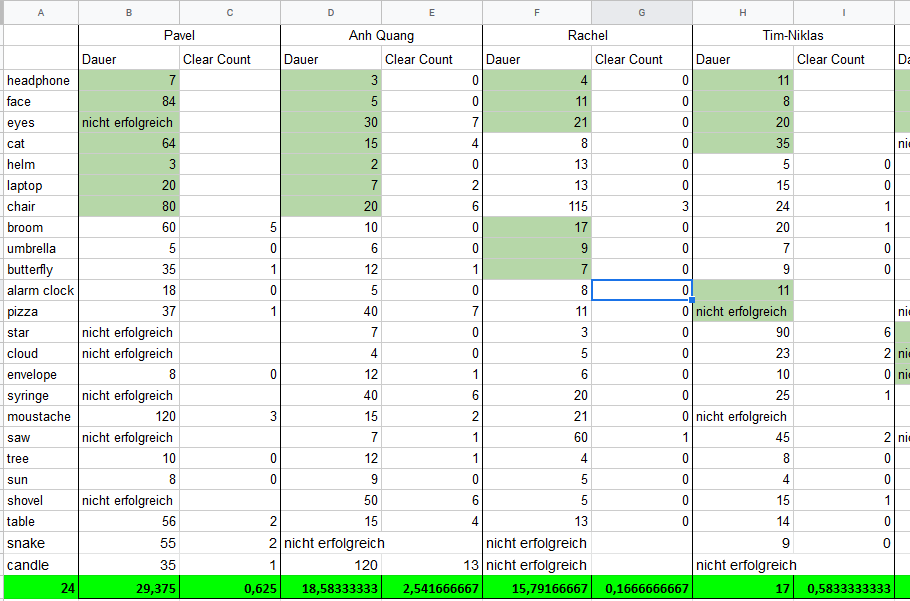
\includegraphics[width=1\textwidth]{images/blindtesting.png}
\caption{\label{fig:testResults}Ergebnisse des Testzeichnen}
\end{figure}

Jedesmal wenn die Spieler*in "den Stift absetzt", das bedeutet in unserem Fall, den Finger hebt um neu anzusetzen, soll das gezeichnete an das neuronale Netzwerk übergebenwerden. Dieses berechnet dann die Ergebnisse. Die fünf Ergebnisse mit den höchsten Vorhersagewahrscheinlichkeiten sollen auf dem Spielbildschirm angezeigt werden. Für die Anzeige der fünf wahrscheinlichsten Wörter soll ein Balkendiagramm verwendet werden, welches das Wort und die zugehörige Wahrscheinlichkeit in Prozent zeigt. Außerdem soll, falls das korrekte Wort in der Auswahl enthalten ist, dieses farblich hervorgehoben werden. Am oberen Rand des Spielbildschirms soll ein farblich hervorgehobener Balken anzeigen, wie viel Zeit schon vergangen ist. Wenn die Spieler*in es schafft, eine Zeichnung innerhalb der vorgegebenen Zeit zu erstellen, die das neuronale Netzwerk als das vorgegebene Wort erkennt, dann ist die Runde gewonnen. Das bedeutet, dass das gesuchte Wort in den Vorhersagen des neuronalen Netzwerks die höchste Wahrscheinlichkeit im Vergleich mit den anderen Wörtern haben muss. Verloren ist das Spiel, wenn dies der Spieler*in nicht in der vorgegebenen Zeit gelingt. In beiden Fällen hat die Spieler*in dann die Möglichkeit eine neue Runde mit einem neuen Wort zu starten.

\section{Implementierung}
\subsection{Architektur: JavaScript}
Für die Architektur orientieren wir uns grob am Model View Controller Design Pattern.
\subsubsection{Methodik}
Um eine sinnvolle Architektur für Skribbl.Ai zu entwerfen wurde die Class-Responsibility-Collaboration Card Methode verwendet. Zu sehen in Abbildung \ref{fig:crcCard}. Zunächst wurden mit Hilfe des bereits existierenden Programmcodes Klassen definiert und anschließend die jeweiligen Verantwortlichkeiten und Kollaborationen mit anderen Klassen notiert. Das Resultat dieser Überlegung wurde daraufhin in Programmcode übersetzt und ist in der folgenden Abbildung zu sehen.

\begin{figure}[ht]
\centering
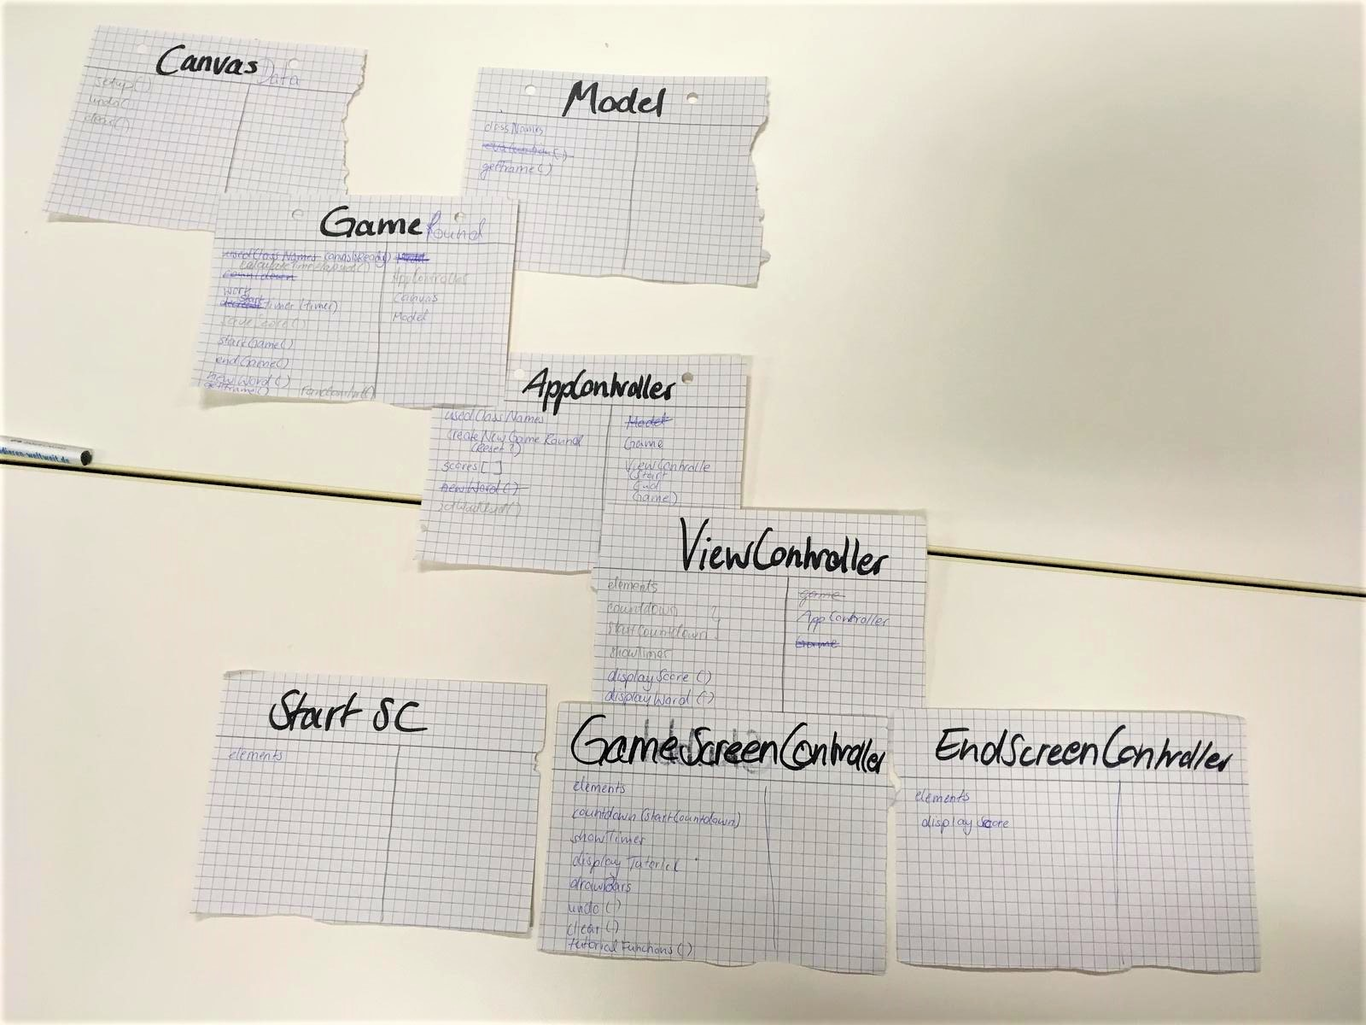
\includegraphics[width=0.75\textwidth]{images/crc.png}
\caption{\label{fig:crcCard}\textit{Class Responsibility Collaborator} Karten}
\end{figure}

\subsubsection{Das Model}
Die Klassen des \textit{Model} sind in Abbildung \ref{fig:classDiagram} blau hinterlegt. Die \textit{CanvasData} Klasse ist zuständig für die Speicherung und Verarbeitung der Daten die auf dem \textit{Canvas} entstehen. Dazu gehören beispielsweise die Maus Koordinaten und das Zuschneiden des gemalten Bildes auf die passende Größe. Die \textit{ModelData} Klasse bindet das neuronale Netzwerk ein und berechnet die Vorhersagen. Die \textit{GameRound} Klasse wiederrum speichert alle Informationen zur aktuellen Spielrunde wie die übrige Zeit und das aktuelle Wort. Die Klassen \textit{Tutorial} und \textit{TutorialStep} sind für die Steuerung durch das Tutorial und die Hervorhebung der betreffenden Bildschirmbereiche verantwortlich. Die \textit{Score} Klasse speichert die Gewinninformationen der Runde.

\subsubsection{Der Applikation Controller}
Die Klasse \textit{AppController} steuert den Verlauf des Spiels. Sie weiß in welchem Status das Spiel sich befindet, welche Wörter schon benutzt wurden und kann neue Runden starten. Da wir für unsere Applikation immer nur einen \textit{AppController} benötigen ist dieser als \textit{Singleton} implementiert. Hierfür wird eine Instanz der Klasse \textit{AppController} in der Klasse \textit{SingletonAppController} gekapselt. Die Klasse \textit{SingletonAppController} ist nur dafür zuständig zu prüfen, ob bereits eine Instanz von \textit{AppController} existiert und gegebenenfalls eine Neue zu erstellen oder die Existierende zurück zu geben. \textit{AppController} und \textit{SingletonAppController} sind in Abbildung \ref{fig:classDiagram} grün hinterlegt.

\subsubsection{Der View Controller}
Es gibt eine \textit{ViewController} Klasse, diese initialisiert den \textit{AppController} als Feld. Von dieser Klasse erben die Klassen \textit{StartScreenController}, \textit{GameScreenController} und \textit{EndScreenController}, alle vier Klassen sind in Abbildung \ref{fig:classDiagram} rot hinterlegt. Die Kindklassen repräsentieren jeweils einen Spielstatus und sind zuständig die korrekten Bildschirmbereiche anzuzeigen und die dazugehörigen Funktionalitäten zur Verfügung zu stellen. Hierzu gehören die Spracheinstellung auf dem Startbildschirm oder \textit{undo} und \textit{clear} auf dem Bildschirm des Hauptspiels.

\begin{figure}[ht]
\centering
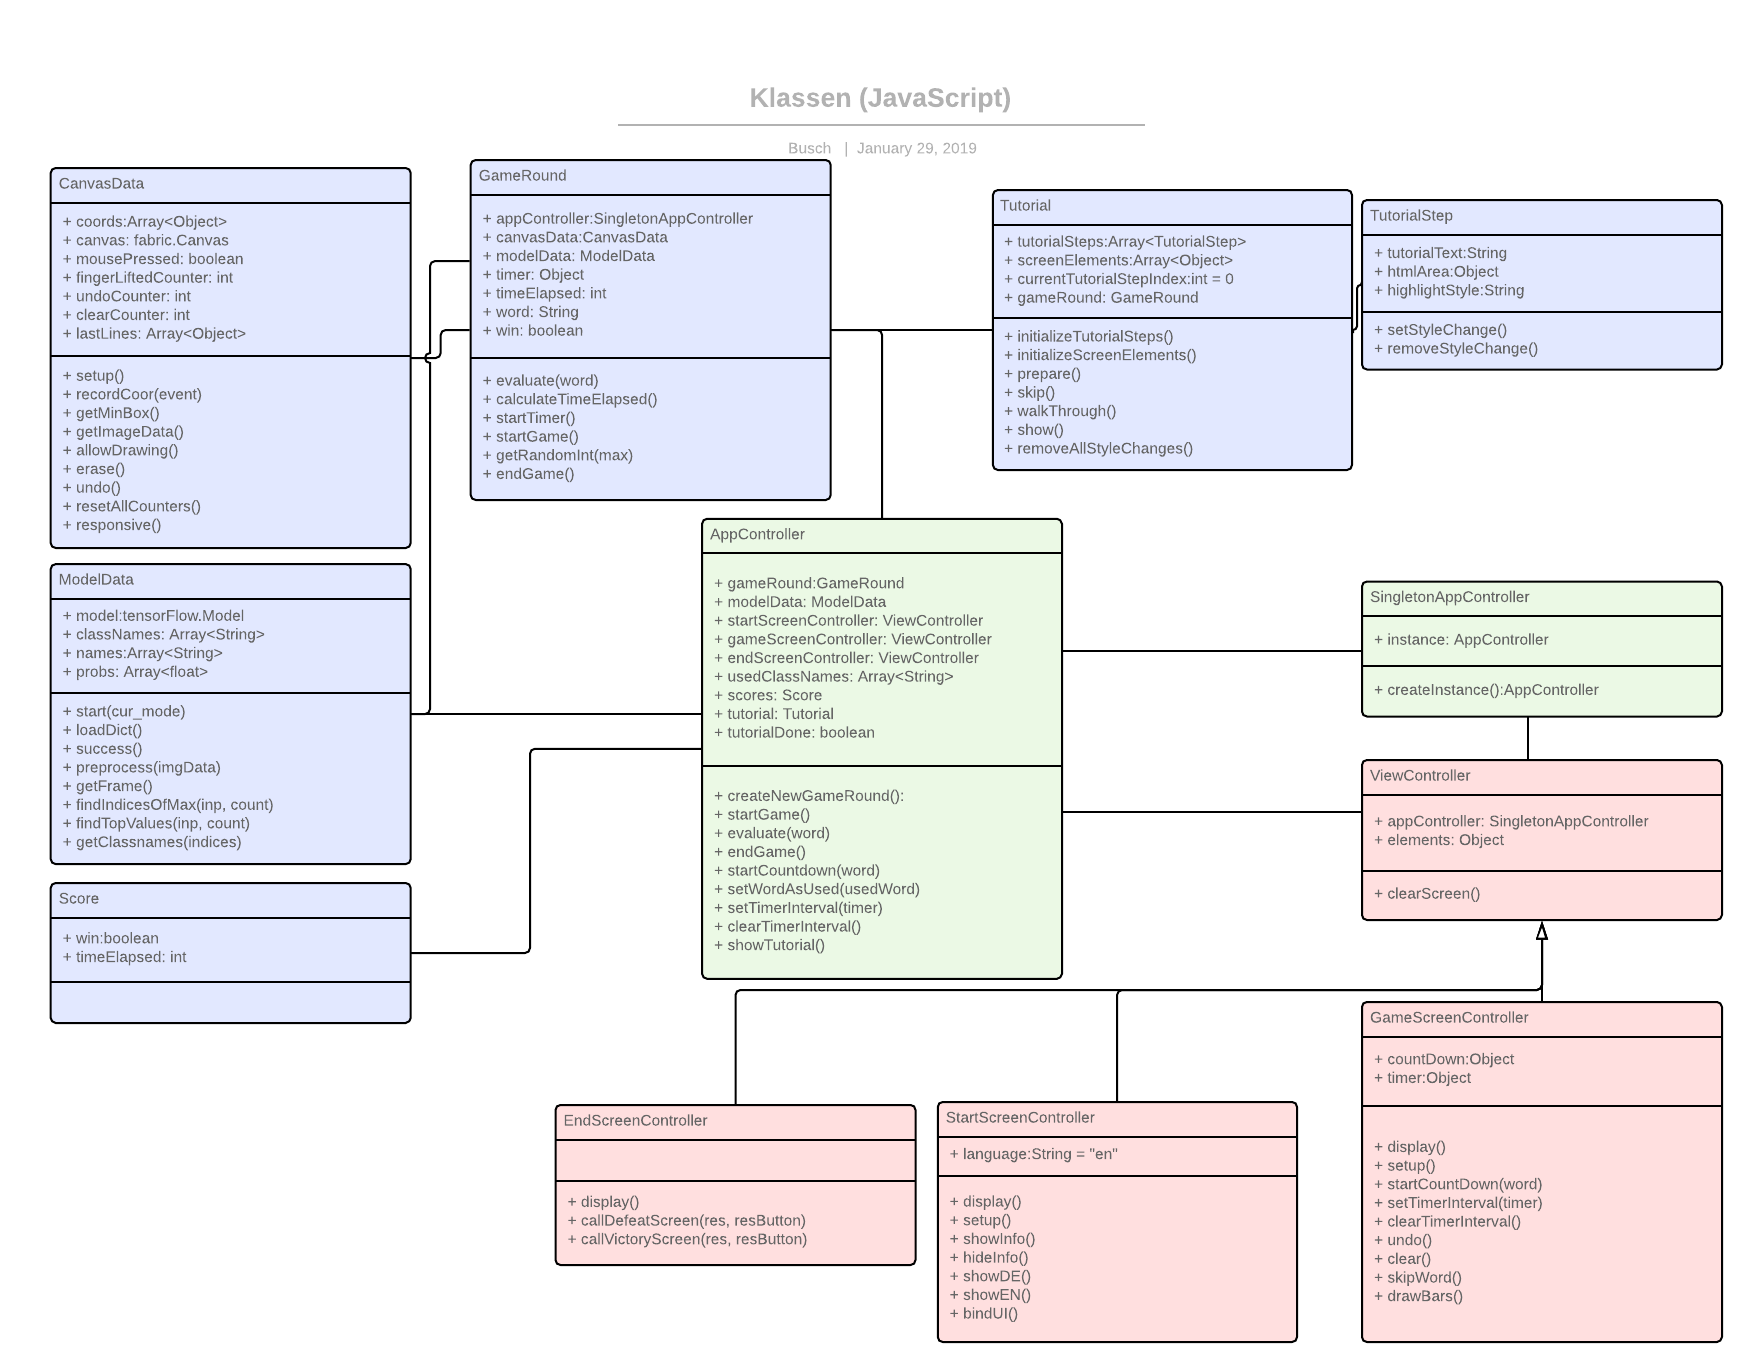
\includegraphics[width=1\textwidth]{images/classDiagramSkribbl.png}
\caption{\label{fig:classDiagram}Klassen Diagramm}
\end{figure}

\section{Spielbeschreibung, Ziel}

\iffalse
Spielkonzept ist bereits beschrieben in Anforderung, Spielkonzept
\fi

\section{Bewertung}
vgl. Anforderungen mit Ergebnis
\pagebreak

\section{Anlangen}
\label{chap: Anlagen}
\subsection{Styleguide}


\textbf{General Rules}
\begin{itemize}
\item Daten sollten so gut wie möglich und so oft wie möglich in Diagrammen und Bildern dargestellt werden
\item Text sollte bis auf 200\% herangezoomt werden können \item Bilder sollten einen Alt-Data Text haben\\
\end{itemize}

\textbf{Buttons}
\begin{itemize}
\item sollten einen ausreichenden Farb-Kontrast haben
\item Kurz angebunden
\item Abkürzungen gerne, aber sie sollten entweder aus einem Idiom bestehen oder einmal erklärt worden sein\\
\end{itemize}

\textbf{Formattierung}
\begin{itemize}
\item Klammer-Paare sollten vertikal immer Matching Braces should always line up vertically in the same column as their constructall if, while and for statements must be written with parentheses, even if they only carry one condition
Binary operators should have one space on each side
\item Parenthesis' should be used in expressions not only to clarify but also to simplify
\item Klassennamen starten mit einem Großbuchstaben (Camelcase ist erlaubt wenn notwendig)
\item Alle anderen identifiers starten klein geschrieben und benutzen daraufhin Camelcase (keine Leerzeichen)\\
\end{itemize}

\textbf{Coding}
\begin{itemize}
\item Jede Methode sollte etwas zurück geben
\item Es wird kein Continue benutztbreak wird nicht außerhalb eines switch-cases benutzt
\item Variablen werden so nahe wie möglich am Ort ihrer Benutzung initialisiert
\item Public Variablen so wenig wie nötig benutzen\\
\end{itemize}

\textbf{Farben}

\begin{tabular}{llll}
\#7ed957    grün & \#FF2E2E    rot & \#4265ff    blau & \#ffde59    gelb \\
\#545454    dunkleres grau & \#737373    dunkelgrau & \#a6a6a6    hellgrau & \#d9d9d9    sehr helles grau\\
\end{tabular}
\pagebreak

\begin{large}\textbf{Schrift}\end{large}
\begin{itemize}
\item Schriftgröße: Entweder 18 px oder 14 px und fett (Je nach Media Queries und Layout)
\item Schriftstyle: non-serif, non-monospace
\item Schriftart: Standard Browser Schriftart (Norwester für das Logo-font)\\
\end{itemize}

\textbf{Sprache}
\begin{itemize}
\item Einfache Sprache
\item English/Deutsch(Wörter)\\
\end{itemize}

\pagebreak
\printbibliography
\end{document}
